\documentclass[aspectratio = 169]{beamer}
\usepackage[english]{babel}
\usetheme{Berkeley}
\usepackage{graphicx}
\DeclareMathOperator*{\argmax}{arg \, max}

\author{Jack Yang}
\title{Linear Discriminant Analysis}
\date{\today}

\begin{document}

\frame[plain]{\titlepage}

\begin{frame}

\frametitle{Outline}
\tableofcontents

\end{frame}

\section{Classification}

\begin{frame}
\frametitle{Classification}

What is Classification?

% \pause

\vspace{0.4cm}

Classification is assigning a $d$-dimensional data point to one of a discrete number of classes.

% \pause

\vspace{0.4cm}

Building a Classifier

% \pause

\begin{itemize}

% \pause

\item Generative Models (e.g., Linear Discriminant Analysis)

% \pause

\item Discriminative Models (e.g., Logistic Regression)

% \pause

% \item Find Decision Boundary (e.g., Support Vector Machine)

\end{itemize}

\end{frame}

\subsection{Building a Classifier}

\begin{frame}

\frametitle{Generative Models}

Given the training data, we want to generate new samples from same distribution.

\vspace{0.4cm}

\begin{centering}

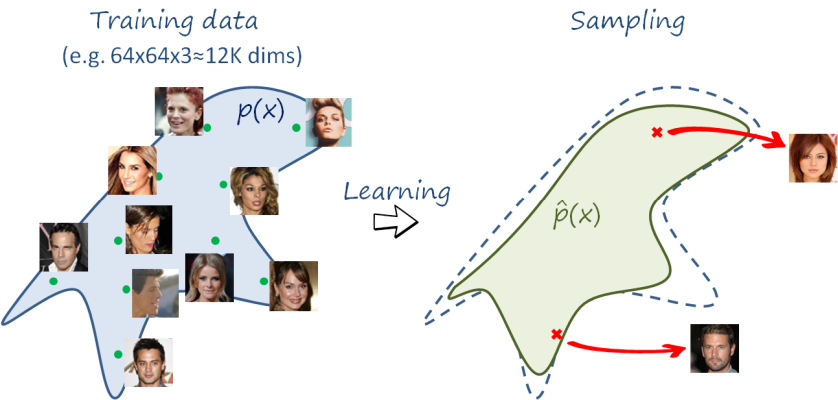
\includegraphics[scale = 0.5]{Figures/generative.png}

\end{centering}

Assume $\text{Training Data} \sim p_{\text{data}} (x)$ and $\text{Generating Data} \sim p_{\text{model}} (x)$, we want to learn $\text{Generating Data} \sim p_{\text{model}} (x)$ similar to $\text{Training Data} \sim p_{\text{data}} (x)$.

% Generative models have strong roots in probabilistic modeling.

% \pause

% \begin{itemize}

	% \item Assume sample points come from probability distributions, different for each class.

	% \pause

	% \item Guess form of distributions.

	% \pause

	% \item For each class $C$, fit distribution parameters to class $C$ points, giving $\mathbb{P}(X \vert Y = C)$.

	% \pause

	% \item For each $C$, estimate $\mathbb{P}(Y = C)$. Bayes' Theorem gives $\mathbb{P}(Y \vert X)$.

	% \pause

	% \item Pick class $C$ that maximizes $\mathbb{P}(Y = C \vert X = x)$, the posterior probability.

% \end{itemize}

\end{frame}

% \subsection{Discriminative Models}

\begin{frame}

\frametitle{Discriminative Models}

Discriminative models directly learn a decision boundary.

% \pause

\vspace{0.4cm}

\begin{centering}

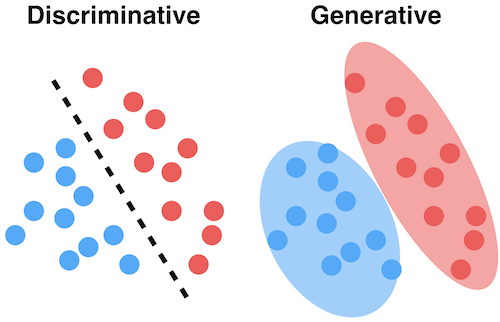
\includegraphics[scale = 0.4]{Figures/discriminative.png}

\end{centering}

% Two ways 

% \begin{itemize}

	% \item Form a posterior distribution $\mathbb{P}(Y \vert X)$ without considering the prior or conditional distributions, that is, to choose a class hat maximizes the posterior probability distribution 
	% $$
	% \hat{y} = \argmax_k \mathbb{P}(Y = k \vert X).
	% $$

	% \pause

	% \item Directly form a hard decision boundary without considering any probabilities in the first place.

% \end{itemize}

\end{frame}

% \subsection{Direct Decision Boundary}

% \begin{frame}

% \frametitle{Decision Boundary}

% \end{frame}

\section{Lienar Discriminant Analysis}

\begin{frame}

\frametitle{Linear Discriminant Analysis}

Intuitively, a good classifier is one that bunches together observations in the same class and separates observations between classes.

\vspace{0.4cm}

% \pause

\begin{itemize}

	\item Fisher's Linear Discriminant attempts to do this through dimensionality reduction.

	% \pause

	\begin{itemize}

		\item Specifically, it projects data points onto a single dimension and classifies them according to their location along this dimension.

	\end{itemize}

	% \pause

	\item Bayes' Linear Discriminant attempts to do this through probabilistic modeling.

\end{itemize}

\end{frame}

\subsection{Fisher's Linear Discriminant}

\begin{frame}

\frametitle{Fisher's Linear Discriminant}

Separate samples of distinct groups by projecting them onto a space that 

\begin{itemize}

	\item Maximizes their between-class separability while

	\item Minimizing their within-class variability

\end{itemize}

% \pause

\vspace{0.4cm}

\begin{centering}

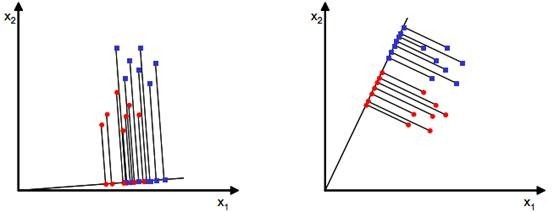
\includegraphics[scale = 0.5]{Figures/fisher.jpg}

\end{centering}

\end{frame}

\begin{frame}

\frametitle{Approach: Maximize Class Separation}

Assume we have $d$-dimensional samples $\{x_1, x_2, \ldots, x_N \}$. We seek to obtain a scalar $y$ by projecting the samples $x$ onto a line. 

\vspace{0.4cm}

% \pause

Consider two classes: $C_1$ with $N_1$ points and $C_2$ with $N_2$ points.

% \pause

\begin{itemize}

	\item The corresponding mean vectors  
	$$
	\mu_1 = \frac{1}{N_1} \sum_{n \in C_1} x_n \qquad \mu_2 = \frac{1}{N_2} \sum_{n \in C_2} x_n.
	$$

	% \pause

	\item Measure class separation as the distance of the projected class 
	$$
	\left|\tilde{\mu_2} - \tilde{\mu_1} \right| = \left|w^T \mu_2 - w^T \mu_1 \right| = \left|w^T (\mu_2 - \mu_1) \right|
	$$
	where $w$ is the projection vectors used to project $x$ to $y$ and we want to maximize this with respect to $w$ with the constraint $\|w \| = 1$.

	% \pause

\end{itemize}

\end{frame}

\begin{frame}

\frametitle{Approach: Minimize Within-Class Variability}

We want to maximize their between-class separability \textbf{and} minimize their within-class variablity.

\vspace{0.4cm}

% \pause

For each class $C_k$, the \textbf{within-class scatter} is given as 
$$
s_k = \sum_{n \in C_k} (y_n - \tilde{\mu_k})^2
$$
where $y_n = w^T x_n$ and $\tilde{\mu_k} = w^T \mu_k$.

% \pause

\end{frame}

\begin{frame}

\frametitle{Maximize Fisher Criterion}

Let 
$$
J(w) = \frac{\text{Between-Class Scatter}}{\text{Within-Class Scatter}} = \frac{\left(\tilde{\mu_2} - \tilde{\mu_1} \right)^2}{s_1^2 + s_2^2} = \frac{w^T S_B w}{w^T S_W w}
$$
where 
$$
S_B = (\mu_2 - \mu_1) (\mu_2 - \mu_1)^T, \quad S_W = \sum_k \sum_{n \in C_k} (x_n - \mu_k)(x_n - \mu_k)^T.
$$

% \pause

By Lagrange Multiplier, we will finally get 
$$
w = S_W^{-1} \left(\hat{\mu_2} - \hat{\mu_1} \right).
$$

\end{frame}

\subsection{Bayesian Approach to LDA}

\begin{frame}

\frametitle{Naive Bayes}

Naive Bayes, is a classifier based on Bayes Theorem with the ``naive'' assumption that features are independent of each other.

% \pause

\vspace{0.4 cm}

\begin{theorem}[Bayes' Theorem]

Given a feature vector $X = (x_1, x_2, \ldots, x_n)$ and a class variable $C_k$, 
$$
\mathbb{P}(C_k \vert X) = \frac{\mathbb{P}(X \vert C_k) \mathbb{P}(C_k)}{\mathbb{P}(X)}
$$
for $k = 1, 2, \ldots, K$.

We call $\mathbb{P}(C_k \vert X)$ the posterior probability, $\mathbb{P}(X \vert C_k)$ the likelihood, $\mathbb{P}(C_k)$ the prior probability of class, and $\mathbb{P}(X)$ the prior probability of predictor.

\end{theorem}

\end{frame}

\begin{frame}

\frametitle{Naive Independence Assumption}

The likelihood function can be decomposed as 
$$
\begin{aligned}
	\mathbb{P}(X \vert C_k) & = \mathbb{P}(x_1, x_2, \ldots, x_n \vert C_k) \\ 
	& = \mathbb{P}(x_1 \vert x_2, \ldots, x_n, C_k) \cdot \mathbb{P}(x_2 \vert x_3, \ldots, x_n, C_k) \cdots \mathbb{P}(x_{n - 1}, x_n \vert C_k) \cdot \mathbb{P}(x_n \vert C_k).
\end{aligned}
$$

% \pause

With the naive conditional independence assumption, that is, 
$$
\mathbb{P}(x_i \vert x_{i + 1}, \ldots, x_n, C_k) = \mathbb{P}(x_i \vert C_k). 
$$

% \pause

Now, the likelihood is $\mathbb{P}(X \vert C_k) = \displaystyle \prod_{i = 1}^n \mathbb{P}(x_i \vert C_k)$. Therefore, the posterior probability can be evaluated as 
$$
\mathbb{P}(C_k \vert X) = \frac{\mathbb{P}(C_k)}{\mathbb{P}(X)} \cdot \prod_{i = 1}^n \mathbb{P}(x_i \vert C_k).
$$

% \pause

\end{frame}

\begin{frame}

\frametitle{Naive Bayes Model}

Since the prior probability of predictor $\mathbb{P}(X)$ is constant, we can get the following proportional relation 
$$
\mathbb{P}(C_k \vert X) \propto \mathbb{P}(C_k) \prod_{i = 1}^n \mathbb{P}(x_i \vert C_k).
$$

% \pause

Now, we want to find a class $\hat{C}$ that maximizes the posterior probability, 
$$
\hat{C} = \argmax_{C_k} \mathbb{P}(C_k) \prod_{i = 1}^n \mathbb{P}(x_i \vert C_k).
$$

Further, we may use Maximum Likelihood Estimate to find which class it should be.

\end{frame}

\end{document}